\documentclass[a4paper]{article} % Document type
\ifx\pdfoutput\undefined
    %Use old Latex if PDFLatex does not work
   \usepackage[dvips]{graphicx}% To get graphics working
   \DeclareGraphicsExtensions{.eps} % Encapsulated PostScript
 \else
    %Use PDFLatex
   \usepackage[pdftex]{graphicx}% To get graphics working
   \DeclareGraphicsExtensions{.pdf,.jpg,.png,.mps} % Portable Document Format, Joint Photographic Experts Group, Portable Network Graphics, MetaPost
   \pdfcompresslevel=9
\fi
\usepackage{amsmath,amssymb}   % Contains mathematical symbols
\usepackage[ansinew]{inputenc} % Input encoding, identical to Windows 1252
\usepackage[english]{babel}    % Language
\usepackage[round,authoryear]{natbib}  %Nice author (year) citations
%\usepackage[square,numbers]{natbib}     %Nice numbered citations
%\bibliographystyle{unsrtnat}           %Unsorted bibliography
\bibliographystyle{plainnat}            %Sorted bibliography

\addtolength{\topmargin}{-20mm}% Removes 30mm from the top margin
\addtolength{\textheight}{10mm}% Adds it to the text height
\usepackage{indentfirst}

\begin{document}               % Begins the document

\title{Automatic creation of metadata/markup by use of natural language processing of full text articles}
\author{First name Last name \\ student number \\ email} 
%\date{2010-10-10}             % If you want to set the date yourself.

\maketitle                     % Generates the title

\section*{overview}
\label{sec:prob}

We�re producing a program which automatically generate metadata such as authors� name, date of publishing, name of articles� and more importantly auto-abstract for full text articles
We are interested in features for either more convenient use of the program or improving precise data generation
There are 5 related problems.\\
\begin{figure}
	\caption{The process of metadata creation}
\begin{center}
	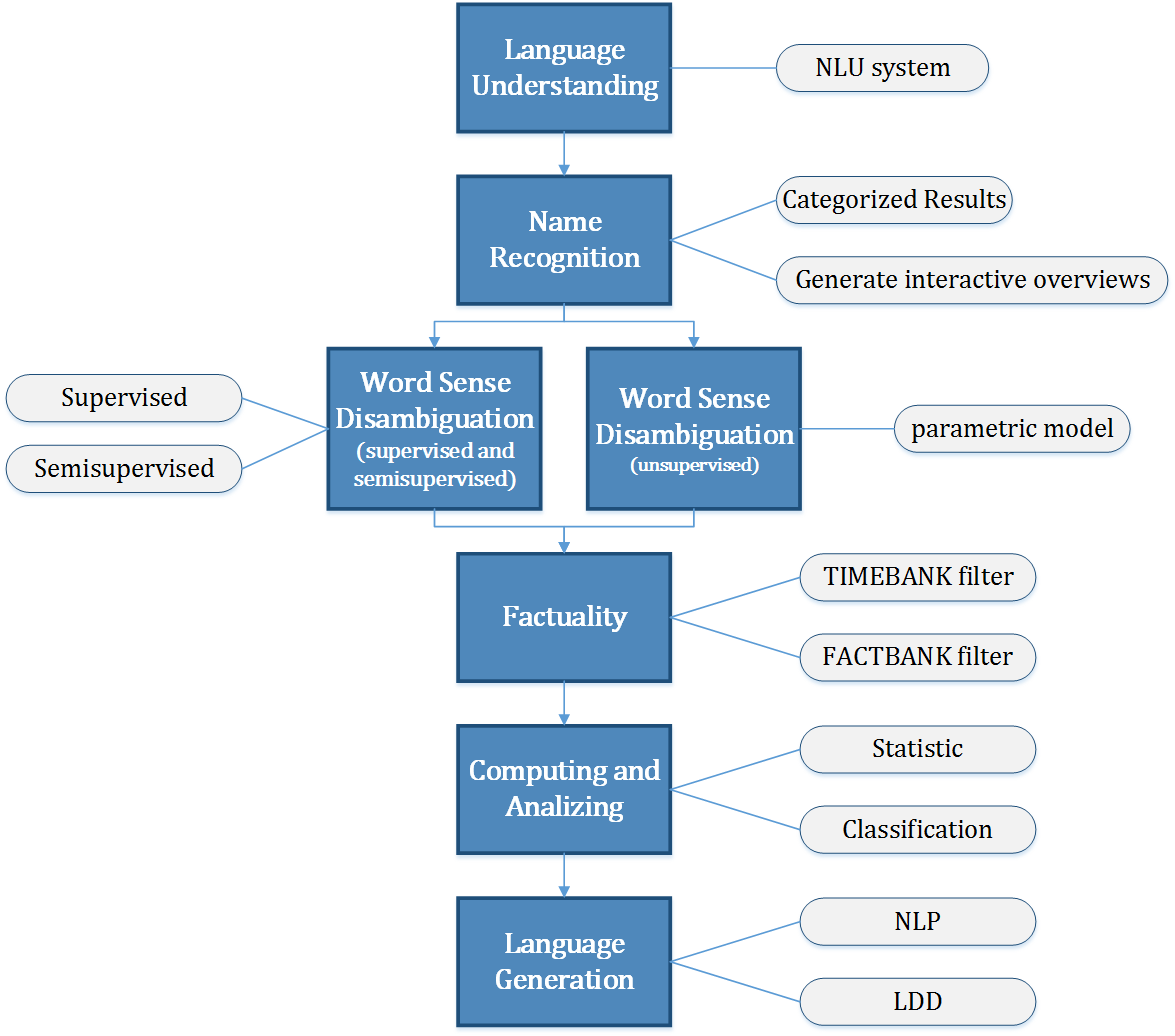
\includegraphics[width=\textwidth]{UnionChart}
\end{center}
\end{figure}

\section*{Language understanding}

When  users  search  with  a  sentence,  how  do  the  program  understand  the  certain  input  of  text? \\

Building  a  natural  language  understanding  (NLU)  system. Use  a  set  of  possible  yes-no  questions  that  can  be  applied  to  data  items,  then  follow  a  rule  for selecting  the  best  question  at  any  node  on  the  basis  of training  data,  which  has  a  method  for  pruning trees to prevent over-training.


\section*{Name Recognition}
The results could be a country or an animal if users search for the word, Turkey. Sometimes, the results are totally unrelated. That would be troublesome when we count frequency of a certain word to rank it. 
Therefore, it�s significantly crucial for search engine to understand what users want by name recognition in natural language processing. The users can find out the results much quicker and can�t get misunderstood.
The method to improve the above problem is �categorize the results based on different subjects or genres� by using online database. Digital libraries and web resources have limited metadata, augmenting them with meaningful, stable and desired categories.(Bill2006, Categorizing Web Search Results into Meaningful and Stable Categories Using Fast-Feature Techniques)
Information can enable better overviews and support user exploration. It will be very convenient to find the results we want.( Jin2008, Effectiveness Web Search Results for Genre and Sentiment Classification) Users don�t have to filter the results which are ranked by browsing frequency. Users just can obtain the information and relevance by clicking the specific categories. 
Creating and using an online database or automated metadata creation are to be recommended. The reason why is because there are some advantages, including integrating with the other cloud service or scaling with what users need such as how to categorize the categories.\\


\section*{Word sense disambiguation: supervised and semi-supervised approach}

Word sense disambiguation (WSD) is an open problem of natural language processing and ontology. WSD is identifying which sense of a word (i.e.meaning) is used in a sentence, when the word has multiple meanings. The solution to this problem impacts other computer-related writing, such as discourse, improving relevance of search engines, anaphora resolution, coherence, inference et cetera.
The human brain is quite proficient at word-sense disambiguation. The fact that natural language is formed in a way that requires so much of it is a reflection of that neurologic reality. In other words, human language developed in a way that reflects (and also has helped to shape) the innate ability provided by the brain's neural networks. In computer science and the information technology that it enables, it has been a long-term challenge to develop the ability in computers to do natural language processing and machine learning.
\subsection*{Supervised}
Supervised methods are based on the assumption that the context can provide enough evidence on its own to disambiguate words (hence, common sense and reasoning are deemed unnecessary). Probably every machine learning algorithm going has been applied to WSD, including associated techniques such as feature selection, parameter optimization, and ensemble learning. Support Vector Machines and memory-based learning have been shown to be the most successful approaches, to date, probably because they can cope with the high-dimensionality of the feature space. However, these supervised methods are subject to a new knowledge acquisition bottleneck since they rely on substantial amounts of manually sense-tagged corpora for training, which are laborious and expensive to create.
\subsection*{Semi-supervised}
Because of the lack of training data, many word sense disambiguation algorithms use semi-supervised learning, which allows both labeled and unlabeled data. The Yarowsky algorithm was an early example of such an algorithm.[24] It uses the �One sense per collocation� and the �One sense per discourse� properties of human languages for word sense disambiguation. From observation, words tend to exhibit only one sense in most given discourse and in a given collocation.\\
The bootstrapping approach starts from a small amount of seed data for each word: either manually tagged training examples or a small number of surefire decision rules (e.g., 'play' in the context of 'bass' almost always indicates the musical instrument). The seeds are used to train an initial classifier, using any supervised method. This classifier is then used on the untagged portion of the corpus to extract a larger training set, in which only the most confident classifications are included. The process repeats, each new classifier being trained on a successively larger training corpus, until the whole corpus is consumed, or until a given maximum number of iterations is reached.\\
Other semi-supervised techniques use large quantities of untagged corpora to provide co-occurrence information that supplements the tagged corpora. These techniques have the potential to help in the adaptation of supervised models to different domains.\\
Also, an ambiguous word in one language is often translated into different words in a second language depending on the sense of the word. Word-aligned bilingual corpora have been used to infer cross-lingual sense distinctions, a kind of semi-supervised system.
\subsection*{Unsupervised}
Word sense disambiguation (WSD) is a core research problem in computational linguistics and natural language processing (NLP), which was recognized since the beginning of the scientific interest in machine translation, and in artificial intelligence, in general. Finding a solution to the WSD problem is in many cases essential, or even compulsory, either for natural language understanding, or for a wide range of applications such as: information retrieval, machine translation, speech processing, text processing etc. From the wide range of unsupervised learning techniques that could be applied to our problem, we have chosen to use a parametric model in order to assign a sense group to each ambiguous occurrence of the target word. The disambiguation method using N-gram features that is being presented here is unsupervised and uses counts collected from the web in a simple way, in order to rank candidates. It does not require sense definitions or inventories; the only requirement is for these counts to be available. \\

Word sense disambiguate is an open challenge in NLP, many researches are in progress, to find the correct sense of a given word. Each word will have different senses, the sense of the word purely depends on the particular context, so that a word can be interpreted in more than one way. The main motivation is to avoid word sense disambiguation and to make ample use of available technologies, so as to achieve this, many approaches are there.\\
\section*{Factuality}
In the process of producing metadatas, which are should be the most precise information and representing the text, validity of such metadata must be checked. Therefore tools for fact checks are developed based on linguistic techniques.  The tool could detect facts and excludes authors� subjective opions (Agerri et al., 2015). From this paper�s perspective, the two main set of tools having such functions is TIMEBANK and FACTBANK.
TIMEBANK was first proposed in 2003 (Pustejovsky et al., 2003). The idea was based on that English language has different tenses which could be exploited as signals for fact check. An example as below could help clarifying the ideas. Let�s examine these sentence:\\
\begin{flushleft}
	-	I will go to Chimei museum tomorrow.\\
	-	Chimei museum is near Tainan District.\\
	-	I was in UK in 2012.\\
\end{flushleft}

The first sentence is simple future tense which implying something has never actually happened, the second sentence is simple present tense which can directly imply facts, and the last sentence is in simple past tense which is about something already happened (which is facts), but is no longer a fact right now � so such fact must be used with caution. \\

In addition to TIMEBANK, many other tools can be another filter for fact extraction. The reason for introducing such tool is that even scientific reseach articles can be glittering with subjective comments, opions or even assumption from authors (Schultze, 2000). (Dave et al., 2003) identify words, clauses and phrases that show emotional state of the authors. The choice in expression of facts could also be a helpful indicator to show whether authors are sujectively supporting a cause, an opion and so on (Wiebe et al., 2005). Among these mentioned approaches, this paper highly favors creation a kind of thesaurus compiled of linguistic signalling for non-factually statementssuch as FACTBANK, which is built by (Saur� and Pustejovsky, 2009). Following example shows how subjective statements can be picked out.\\
\noindent
\begin{flushleft}
	   -   Channelization would guarantee high flow velocity in rivers, more flooding and consequent degradation of riparian community (1 a)\\
	   -	Funding angencies would be happy with big entrepreneurs, instead of small and medium enterprises. (1 b)\\
	   -	Tolerance to dictatorship would has negative influences on anarchist movement (2 a)\\
	   -	Tolerance to dictatorship would doom anarchist movement. (2 c)\\
\end{flushleft}

It is easy to find in statement (1 a) is an absolute fact. Statement (1 b) is howerver affected by emotional state of authors. After re-writting (1 b) into: Funding agencies lend more money with lower interest rate to big entrepreneurs, instead of small and medium enterprises, sentence (1 b) become a face-based statement. In another case, statement (2 a) is a fact-based statement while in statement (2 b), authors are stressing their dislike toward dictatorship.\\
Fact checks in language generation is a new field but many useful tool has been developed. Each of them has their own function and could complement each others. In the limit of this study, we are using both of TIMEBANK and FACTBANK together for fact check. \\

\section*{Computing and analysing}
I suggest we should use the Python language to complete this task. 
It can easily conpute and analyze the words in the articles.
Phthon can compute and analyze by separating the connected words.
The readers can know what do the words mean when they are reading the articles .

\section*{Direction}
\label{sec:prob}


In order to highlight the focus of the article ,the special and important words in the article need to be found mostly.
The article will promote these words to make the article's mainpoint prominent.
Compute all the words in the article and show the number of occurrences of most rankings.
By these words ,the analyzer know which words in the article should be analyzed.


\section*{Operate}
\label{sec:meth}
1. distinguish     : distinguish all the words in the article\\\\
\begin{center}
	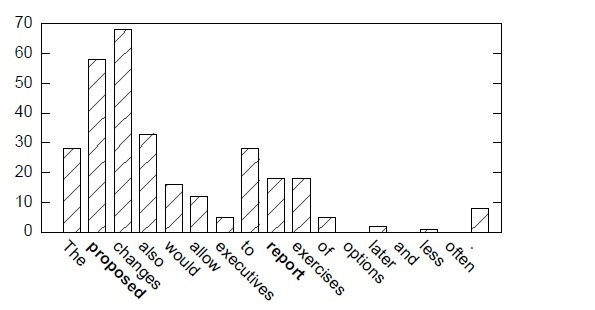
\includegraphics[scale=1.0]{union_01.jpg}
\end{center}
2. classification   : Divided into four categories by word count.\\


a. Word Count $>$ 15 

b.15 $>$ Word Count $>$ 10

c. 10 $>$ Word Count $>$5 

d. 5 $>$Word Count

\begin{center}
	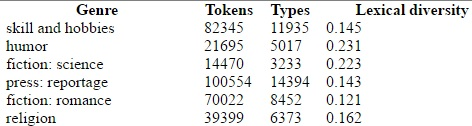
\includegraphics[scale=1.5]{union_02.jpg}
\end{center}
3. search       : Search Word repetition rate in the article.\\
4. statistics     : count the repetition rate of words in the article.\\
5. sort         : Show the  number of occurrences of most rankings in every categorie.\\




\section*{Language generation}
\label{sec:prob}
Natural language processing help us extract the important information from the full text article.
How could we make it more efficiently and precisely?
Query reduction to single sub-query
The performance of the machine is better in the short query rather than long query. Thus, it is an important issue to reduce the query to many sub-query.  The first is extracting the single sub-query by the existing features. Then, We combine these features to the reduction�s technique. We could find that it is more efficient than just analyze the original query. 


\bibliography{Union homework 3}
[1].Jin 2008, Effectiveness Web Search Results for Genre and Sentiment Classification
\\\
[2].Bill 2006, Categorizing Web Search Results into Meaningful and Stable Categories Using Fast-Feature Techniques
\\\
[3].Weiscbedel 2006 White Paper on Natural Language Processing
\\\
[4].Collins 2011 Natural Language Processing Machine Learning Research
\\\
[5].Manish Gupta 2015, Information Retrieval with Verbose Queries, Foundations and Trends in Information Retrieval
\\\
[6].Julia Hirschberg 2015, Advances in natural language processing, Science
\\\
[7].Shapiro1982, A knowledge engineering approach to natural language understanding 
\\\
[8].Kuhn1995, The Application of Semantic Classification Trees to Natural Language Understanding
\\\
[9].Abualhaija, S.and Zimmermann, K.-H. 2016. D-Bees: A novel method inspired by bee colony optimization for solving word sense disambiguation. Swarm and Evolutionary Computation, 27, 188-195.
\\\
[10]. Ben Aouicha, M., Hadj Taieb, M. A.and Ezzeddine, M. 2016. Derivation of �is a� taxonomy from Wikipedia Category Graph. Engineering Applications of Artificial Intelligence, 50, 265-286.
\\\
[11]. Navigli, R. 2009. Word sense disambiguation: A survey. ACM Computing Surveys (CSUR), 41, 10. 
\\\
[12]. Wang, H., Missura, O., G�rtner, T.and Wrobel, S. 2009. Context-based clustering of image search results. In: KI 2009: Advances in Artificial Intelligence. Springer.
\\\
[13]. Yoon, Y., Seon, C.-N., Lee, S.and Seo, J. 2006. Unsupervised word sense disambiguation for Korean through the acyclic weighted digraph using corpus and dictionary. Information Processing and Management, 42, 710-722.
\\\
Agerri, R., Artola, X., Beloki, Z., Rigau, G. and Soroa, A. 2015. Big data for Natural Language Processing: A streaming approach. Knowledge-Based Systems, 79, 36-42.
Dave, K., Lawrence, S. and Pennock, D. M. Mining the peanut gallery: Opinion extraction and semantic classification of product reviews.  Proceedings of the 12th international conference on World Wide Web, 2003. ACM, 519-528.
Pustejovsky, J., Hanks, P., Sauri, R., See, A., Gaizauskas, R., Setzer, A., Radev, D., Sundheim, B., Day, D. and Ferro, L. The timebank corpus.  Corpus linguistics, 2003. 40.
Saur�, R. and Pustejovsky, J. 2009. FactBank: A corpus annotated with event factuality. Language resources and evaluation, 43, 227-268.
Schultze, U. 2000. A confessional account of an ethnography about knowledge work. MIS Quarterly: Management Information Systems, 24, 3-40.
Wiebe, J., Wilson, T. and Cardie, C. 2005. Annotating expressions of opinions and emotions in language. Language resources and evaluation, 39, 165-210.



\end{document}      % End of the document
